\documentclass{article}

% if you need to pass options to natbib, use, e.g.:
%     \PassOptionsToPackage{numbers, compress}{natbib}
% before loading neurips_2019

% ready for submission
% \usepackage{neurips_2019}

% to compile a preprint version, e.g., for submission to arXiv, add add the
% [preprint] option:
%     \usepackage[preprint]{neurips_2019}

% to compile a camera-ready version, add the [final] option, e.g.:
\usepackage[]{neurips_2019}

% to avoid loading the natbib package, add option nonatbib:
%     \usepackage[nonatbib]{neurips_2019}

\usepackage[utf8]{inputenc} % allow utf-8 input
\usepackage[T1]{fontenc}    % use 8-bit T1 fonts
\usepackage{hyperref}       % hyperlinks
\usepackage{url}            % simple URL typesetting
\usepackage{booktabs}       % professional-quality tables
\usepackage{amsfonts}       % blackboard math symbols
\usepackage{nicefrac}       % compact symbols for 1/2, etc.
\usepackage{microtype}      % microtypography


%% added by Hui 
\usepackage{bbm}
\usepackage{mwe}
\usepackage{soul}
\usepackage{subcaption}
\usepackage{cleveref}
\usepackage{graphicx}
\usepackage[english]{babel}
% \usepackage[utf8x]{inputenc}
\usepackage{color}
\usepackage{multirow}
\usepackage{algorithm}
\usepackage{algorithmic}
\renewcommand{\algorithmicrequire}{\textbf{Input:}}
\renewcommand{\algorithmicensure}{\textbf{Output:}}
\newcommand{\algorithmicbreak}{\textbf{break}}
\newcommand{\BREAK}{\STATE \algorithmicbreak}
\renewcommand{\algorithmiccomment}[1]{// #1}
\newtheorem{theorem}{Theorem}
\newtheorem{lemma}{Lemma}
\newtheorem{observation}{Observation}
\newtheorem{definition}{Definition}
\newtheorem{principle}{Principle}
\newcommand{\TODO}[1]{{\it \color{blue}\{TODO: #1\}}}
\newcommand{\MOD}[1]{{\it \color{blue}\{MOD: #1\}}}
\usepackage{mathtools}
\DeclarePairedDelimiter{\ceil}{\lceil}{\rceil}

\usepackage[
  separate-uncertainty = true,
  multi-part-units = repeat
]{siunitx}

\title{In-place Adaptive Near-Zero Cost DNN Protection from Memory Faults}

% The \author macro works with any number of authors. There are two commands
% used to separate the names and addresses of multiple authors: \And and \AND.
%
% Using \And between authors leaves it to LaTeX to determine where to break the
% lines. Using \AND forces a line break at that point. So, if LaTeX puts 3 of 4
% authors names on the first line, and the last on the second line, try using
% \AND instead of \And before the third author name.

\author{%
  David S.~Hippocampus\thanks{Use footnote for providing further information
    about author (webpage, alternative address)---\emph{not} for acknowledging
    funding agencies.} \\
  Department of Computer Science\\
  Cranberry-Lemon University\\
  Pittsburgh, PA 15213 \\
  \texttt{hippo@cs.cranberry-lemon.edu} \\
  % examples of more authors
  % \And
  % Coauthor \\
  % Affiliation \\
  % Address \\
  % \texttt{email} \\
  % \AND
  % Coauthor \\
  % Affiliation \\
  % Address \\
  % \texttt{email} \\
  % \And
  % Coauthor \\
  % Affiliation \\
  % Address \\
  % \texttt{email} \\
  % \And
  % Coauthor \\
  % Affiliation \\
  % Address \\
  % \texttt{email} \\
}

\begin{document}

\maketitle

\begin{abstract}
Deep Neural Networks (DNN) have been successfully applied in many real-world tasks such as self-driving cars and unmanned drones, where it is critical to ensure the reliability of inference results with memory faults.
Traditional methods such as error correction codes (ECC) and Triple Modular Redundancy (TMR) are DNN-agnostic and thus incur non-negligible storage overhead. This paper introduces an adaptive in-place near-zero cost fault protection mechanism that relies on DNN-specific properties to reduce protection overhead while provides the same protection guarantee as ECC. Experiments on three popular DNNs, VGG-16, ResNet18, and SqueezeNet, under various memory fault rates demonstrate the effectiveness of the proposed approach.       


%   The abstract paragraph should be indented \nicefrac{1}{2}~inch (3~picas) on
%   both the left- and right-hand margins. Use 10~point type, with a vertical
%   spacing (leading) of 11~points.  The word \textbf{Abstract} must be centered,
%   bold, and in point size 12. Two line spaces precede the abstract. The abstract must be limited to one paragraph.
\end{abstract}

\section{Introduction}
% DNNs are important
Recent years have witnessed the rapid progress in Deep Neural Networks (DNN) and their successful applications to a wide range of machine learning applications. The demanding computational characteristics of DNNs have led to the popularity of Graphic Processing Units (GPU) and the emergence of various DNN accelerators, such as Google Tensor Processing Units (TPU)~\cite{jouppi2017datacenter} and Eyeriss~\cite{chen2017eyeriss}, for efficient model inferences. 

% memory faults  
While optimizing the performance of DNN inferences has been extensively studied, it remains unclear how reliable the inference results are due to the lack of efficient fault protection mechanisms. One of the major sources of faults in DNN accelerators are memory faults (e.g. bit flip) that can result from several sources such as environment perturbations, temperature variations, voltage scaling, manufacturing defects, wear-out, and radiation-induced soft errors. These faults change the stored data (e.g. DNN parameters), which may cause large deviation of fault-free DNN inference results. As DNNs are increasing adopted in safety-critical fields such as self-driving cars and aerospace, any output deviations may cause catastrophic consequences. Protecting DNNs from memory faults becomes imperative to ensure that the output of DNNs are reliable.   


% prior efforts 
Several general methods are possible to be applied to protect DNNs from memory faults. These methods involve Error Correction Codes (ECC), spatial redundancy, and radiation hardening. However, ECC and spatial redundancy bring large storage overhead. For example, the most commonly used ECC technique, Single Error Correction Double Error Detection (SEC-DED), can correct 1 bit error from a 64-bit data block by introducing eight extra encoding bits. Spatial redundancy requires at least two copies of DNN parameters to correct one error (called Triple Modular Redundancy (TMR)). Radiation hardening is a hardware error mitigation technique that can suffers from non-negligible area overhead. The limitations of these methods make it difficult to efficiently protect DNN from memory faults while not offset the benefits brought by performance optimization.  

One way to address the problem is to design DNN-specific memory fault protection mechanisms that consider the characteristics of DNN algorithms. Prior works in this direction, however, have been focused mainly on the quantification of DNN fault tolerance~\cite{reagen2018ares, li2017understanding} or relied on some error detection/mitigation techniques~\cite{reagen2016minerva, azizimazreah2018tolerating} that have limited protection power or lack performance guarantee.  
% Software-based protection mechanisms that can be easily adopted by general accelerators are not systematically explored yet. 


% our selective protection
This paper introduces an inplace adaptive near-zero cost mechnism to protect DNNs from memory faults. Memory faults are modeled as random bit flips.  
\TODO{ description of our protection methods}



% contribution 
We make the following major contributions:
\begin{itemize}
    \item New insights on DNN fault tolerance.
    \item Effective and near-zero cost mechanism to protect DNN from memory faults.
    \item Extensive experiments on popular DNN models. 
\end{itemize}


\section{Related Work}
%% old work on ANN
There are several studies on fault tolerance of neural networks a few years ago~\cite{phatak1995complete, protzel1993performance, torres2017fault}. While the performance degradation of NNs with various fault models has been discussed, the networks they considered had very different network topologies and much fewer neurons than modern DNNs.  

% recent work on DNN
Fault tolerance of DNNs has recently drawn increasing attentions. 
Li et al.~\cite{li2017understanding} studied the soft error propagation in DNN accelerators and proposed to leverage symptom-based error detectors for detecting errors and a hardware-based technique, selective latch hardening,  for detecting and correcting data-path faults. In \cite{reagen2018ares, arechiga2018the},  some empirical studies were conducted to quantify the fault tolerance of DNNs to memory faults and revealed that DNN fault tolerance varies with respect to model, layer type, and structure. Zhang et al.~\cite{zhang2018analyzing} proposed fault-aware pruning with retraining to mitigate the impact of permanent faults for systolic array-based DNN accelerators (e.g., TPUs). They focused only on faults in the data-path and ignored faults in the memory, which is a different fault model from the one used in this paper.  Qin et al.~\cite{qin2017robustness} studied the performance degradation of 16-bit quantized DNNs under different bit flip rates and proposed to set values of detected erroneous weights as zeros to mitigate the impact of faults. These prior works focused mainly on the characterization of DNN's fault tolerance with respect to various data type and network topologies. While few ad-hoc software-based protection solutions are proposed, they can only detect errors rather than correct them (e.g. detecting extreme values~\cite{li2017understanding}) or have limited protection ability (e.g. setting faulty weights to zero~\cite{qin2017robustness}).        

%% accelerator design: low energy 
A closely related research direction is the design of energy-efficient DNN accelerators by exploiting fault tolerance of DNNs~\cite{temam2012defect, reagen2016minerva, kim2018energy, zhang2018thundervolt}. 
Temam et al.~\cite{temam2012defect} introduced a defect-tolerant energy-efficient neural network accelerator by leveraging the fact that neural networks are intrinsically tolerant to permanent faults after retraining. 
Reagen et al.~\cite{reagen2016minerva} designed a low-power highly-accurate DNN accelerator that optimizes SRAM power by reducing the supply voltage. They leverages active hardware fault detection coupled with bit masking that shifts data towards zero to mitigate the impact of bit flips to DNNs' model accuracy without the need of re-training. 
Similar hardware faults detection techniques are later exploited in \cite{whatmough201714, salami2018resilience, zhang2018thundervolt, hacene2019training} to improve fault tolerance of DNNs. Azizimazreah et al.~\cite{azizimazreah2018tolerating} proposed a novel memory cell designed to eliminate soft errors while achieving a low power consumption.  

% The protection solutions in these works rely on hardware modification to support their hardware-based error detection/mitigation schemes, making them impossible to be applied to general DNN accelerators. 


\section{Problem Statement}
Error Correction Code (ECC) is commonly used in computer systems to correct memory faults. The most popular ECC is an extended hamming code, called Single Error Correction Double Error Detection code (SEC-DED), which corrects a single bit error and detect double bit errors in a 64-bit data block by introducing eight check bits redundancy. A generalization of hamming codes, called Bose, Chaudhuri, and Hocquenghem (BCH), are frequently used for multiple-error correction. Both SEC-DED and BCH can be described as $[n, k, t]$ code for length $n$ codeword, length $k$ data, and $t$-bit error correction. The number of required check bits is $n-k$. Popular SEC-DEC is the $[72,64,1]$ code for single bit error correction and popular BCH is the $[63, 51, 2]$ code for double-error correction. 

Existing ECC protection strategies, however, bring significant storage overhead and are also too rigid to adjust their error correction capacity given available storage budgets. For example, the SEC-DEC $[72, 64, 1]$ code and the BCH $[63, 51, 2]$  have a fixed storage overhead of 12.5\% and 19.0\% respectively. Blindly applying these methods to protect DNN from memory faults contradicts to the spirit of ``squeezing the last bit out'' in the DNN model compression research. 

Our objective is to design adaptive and near-zero cost DNN-specific memory fault protection mechanisms that have the maximum error correction power while meet a limited storage budget. Specially, let $r$ be the memory fault rate, which is the probability of a random bit flip. Let $\mathcal{A}(W)$, $\mathcal{A}(\phi(W, r))$, and $\mathcal{A}_P(\phi(W, r))$ be the accuracy of a DNN model executed in a fault-free memory, a memory with fault rate $r$, and a memory with fault rate $r$ using protection strategy $P$ respectively. The overhead introduced by $P$, $overhead(P)$, is the ratio between the extra space in bytes required to store the check bits and the model size in bytes. Given an overhead budget $B$, Our objective is to find a protection mechanism that reduces accuracy drop due to memory faults:
\begin{align}
    & \min_P \mathcal{A}(W) - \mathcal{A}_P(\phi(W, r)) \nonumber \\
    & s.t. \quad overhead(P) \leq  B. \label{eq:objective}
\end{align}

This work focused on developing protection mechanisms for 8-bit quantized DNN models. The reason are two-folds: 1) 8-bit quantization has been a standard step before model deployment to reduce model size while also providing lower latency with little degradation in model accuracy. 2) Previous studies~\cite{li2017understanding, reagen2018ares} have suggested that DNNs should use data types that provide just-enough numeric value range and precision to increase its fault tolerance. Our explorations on using higher precision including float32 for representing DNN parameters  also show that 8-bit quantized model are the most resilient to memory faults. 


% \subsection{Motivations}
%  The most commonly used Error Correction Code (ECC) in computer systems is SEC-DED, which corrects a single error and detect double errors in 64-bit data block by introducing eight check bits redundancy. Our objective is to design DNN-specific memory fault protection mechanisms such that they provide the same protection guarantee as SEC-DED but with less or even no storage overhead.
% %  
%  We first introduce the necessary background on the SEC-DED technique and then describe the observations that motivate us to develop our inplace SEC-DED protection strategies. 

% \subsection{SEC-DED}
% Single Error Correction Double Error Detection (SECDED) are hamming codes extended with additional parity. 
% Hamming codes are linear codes that can be described as $[n, k]$ for length $n$ codeword and length $k$ data. Let $\overrightarrow{\mathbf{x}}$ be a data block to protect and $\overrightarrow{\mathbf{c}}$ be the corresponding codeword. Both of them are row vectors. A generator matrix, $G$, is a $k\times n$ matrix whose rowspace is the space of codewords. A check matrix, $H$, is a $n \times (n-k)$ matrix that is used to verify the data.  Ideally, $\overrightarrow{\mathbf{c}} = \overrightarrow{\mathbf{x}}G$ and $\overrightarrow{\mathbf{c}}H=0$, where the sum operation is done in modulo-2, if the codeword is error-free. The canonical forms of the generator matrix $G$ and the check matrix are $[I_k | P]$ and $[-P^T | I_{n-k}]$ respectively. The number of check bits added is $m = n - k$. A number of $m$ check bits  can cover at most $2^m -1$ number of bits and thus protect a data block of maximum length $2^m -m -1$ (i.e., $k \leq 2^m -m -1$). 

% Hamming codes have a minimum distance of three, which means that they can detect and correct a single error but cannot distinguish a double bit error from a single bit error. To remedy the shortcoming, SEC-DED extends hamming codes by an extra parity bit. A popular SEC-DED code is $[72, 64]$ code, which has the same space overhead as a $[9, 8]$ parity code. By default, SEC-DEC referred in the paper is the $[72, 64]$ code unless noted differently. 

\section{In-place adaptive near-zero cost protection}
We first describe the observations that motivate us to develop our inplace protection strategies and then elaborate the protection strategies. 

\subsection{Observations}
Our protection strategies are motivated by two major observations.      

\begin{observation}
Weights of a well-trained DNN are mostly small values.
\end{observation}

The row \textit{percentage} in Table~\ref{tab:weight_distribution} shows the value distribution of the absolute value of weights in 8-bit quantized DNN models. The absolute value of more than 99\% of weights are less than 64. Even though eight bits are used to represent each weight value, the number of effective bits to represent values less than 64 is at most seven. The non-informative bits in small values give us the chance to create redundency for correcting errors. 

% Please add the following required packages to your document preamble:
% \usepackage{multirow}
\begin{table}[]
\small 
\centering 
\setlength{\tabcolsep}{0.04cm}
\caption{Accuracy and Weight distribution of 8-bit quantized DNN models on ImageNet. Accuracies are measured using 5K images}
\label{tab:weight_distribution}
\begin{tabular}{|l|l|l|l|l|l|l|l|l|l|}
\hline
\multicolumn{2}{|l|}{Model} & AlexNet & VGG16 & VGG16\_bn & ResNet18 & ResNet34 & Inception\_V3 & DenseNet & SqueezeNet \\ \hline\hline
\multicolumn{2}{|l|}{\#weights} & 61.1M & 138.3M & 138.3M & 11.7M & 21.8M & 27.1M & 28.5M & 1.2M \\ \hline\hline
\multirow{2}{*}{\begin{tabular}[c]{@{}l@{}}Accuracy\\ (\%)\end{tabular}} & Float32 & 64.86 & 79.2 & 80.48 & 76.54 & 79.88 & 77.14 & 83.02 & 67.46 \\ \cline{2-10} 
 & Int8 & 64.8 & 79.36 & 80.14 & 76.46 & 79.88 & 76.58 & 83.04 & 66.86 \\ \hline\hline
\multirow{3}{*}{\begin{tabular}[c]{@{}l@{}}Percentage\\ (\%)\end{tabular}} & {[}0, 32) & 95.09 & 97.69 & 98.84 & 99.56 & 99.72 & 98.23 & 98.79 & 95.16 \\ \cline{2-10} 
 & {[}32, 64) & 4.88 & 2.27 & 1.16 & 0.42 & 0.27 & 1.71 & 1.13 & 4.62 \\ \cline{2-10} 
 & {[}64, 128) & 0.03 & 0.04 & 0.01 & 0.02 & 0.02 & 0.05 & 0.08 & 0.22 \\ \hline
\end{tabular}
\end{table}

% \begin{figure}[H]
% 	\centering
% 	\begin{subfigure}{.42\textwidth}
% 		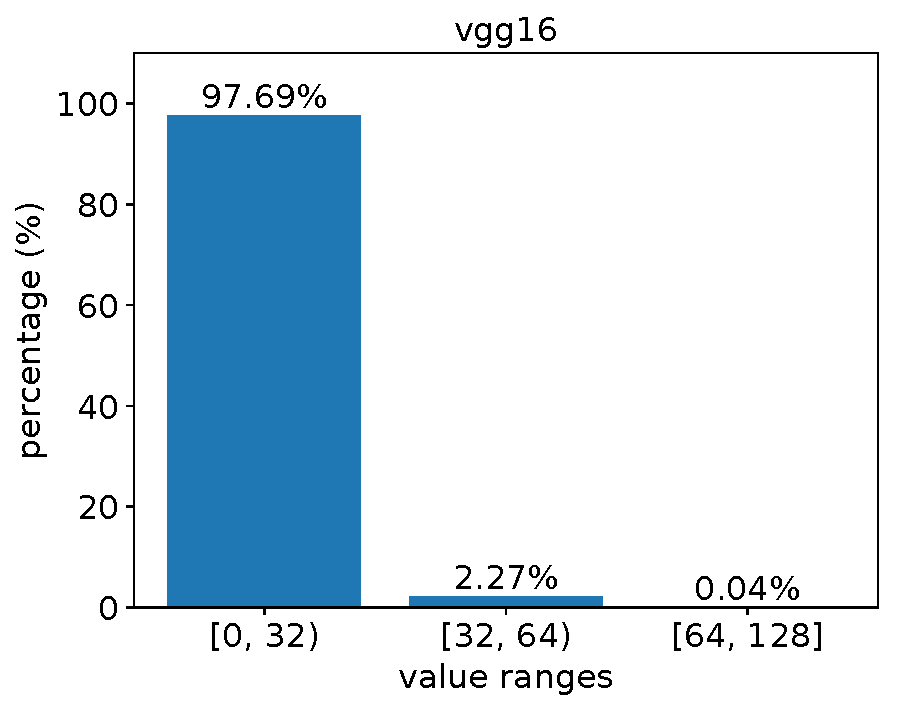
\includegraphics[width=\textwidth]{NeuRIPS2019/images/distribution/vgg16_int8_weight_distribution.pdf}
% 		\caption{VGG16}
% 	\end{subfigure}
% %%%%%%%%%%%%%%
% % 	\begin{subfigure}{.25\textwidth}
% % 		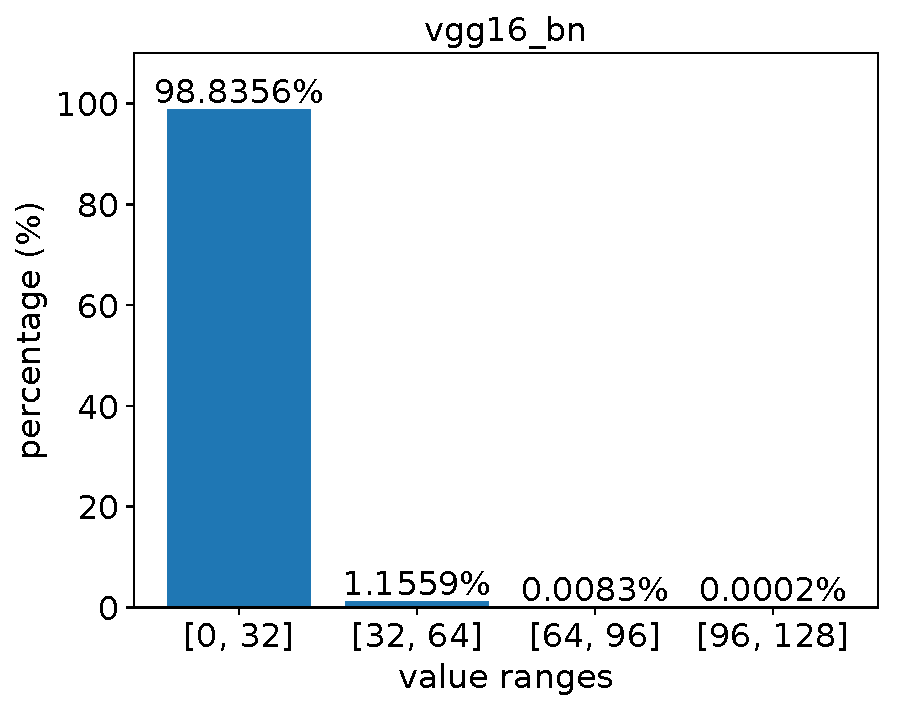
\includegraphics[width=\textwidth]{NeuRIPS2019/images/distribution/vgg16_bn_int8_weight_distribution.pdf}
% % 		\caption{VGG16\_bn}
% % 	\end{subfigure}
% %%%%%%%%%%%%%%
% 	\begin{subfigure}{.42\textwidth}
% 		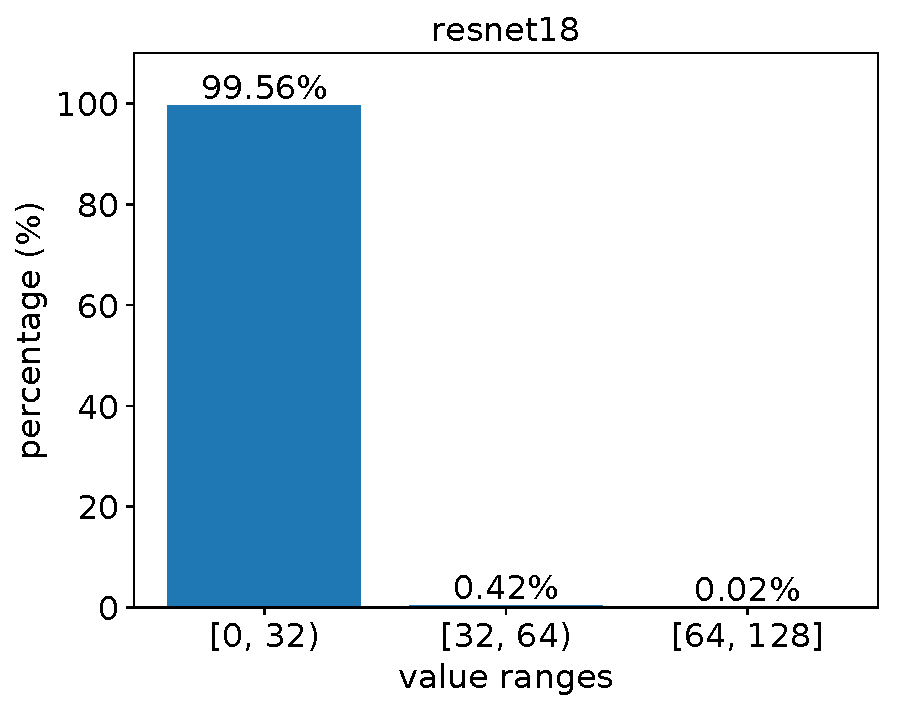
\includegraphics[width=\textwidth]{NeuRIPS2019/images/distribution/resnet18_int8_weight_distribution.pdf}
% 		\caption{ResNet18}
% 	\end{subfigure}
% % 	\begin{subfigure}{.32\textwidth}
% % 		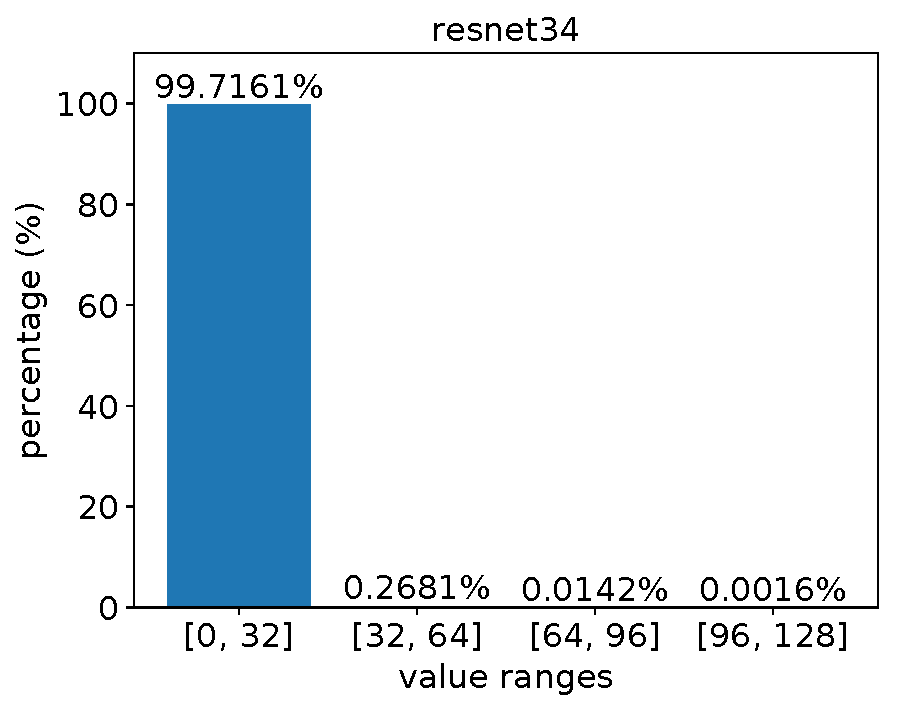
\includegraphics[width=\textwidth]{NeuRIPS2019/images/distribution/resnet34_int8_weight_distribution.pdf}
% % 		\caption{ResNet34}
% % 	\end{subfigure}
% 	\caption{Weight distribution of INT8 quantized DNN models on ImageNet. \TODO{a table with more networks might be better.}}
% 	\label{fig:weight_distribution}
% \end{figure}


\begin{observation}
Low bits, once flipped due to memory faults, cause negaliable or no accuracy drop to DNNs. 
\end{observation}

\begin{figure}
	\centering
	\begin{subfigure}{.42\textwidth}
		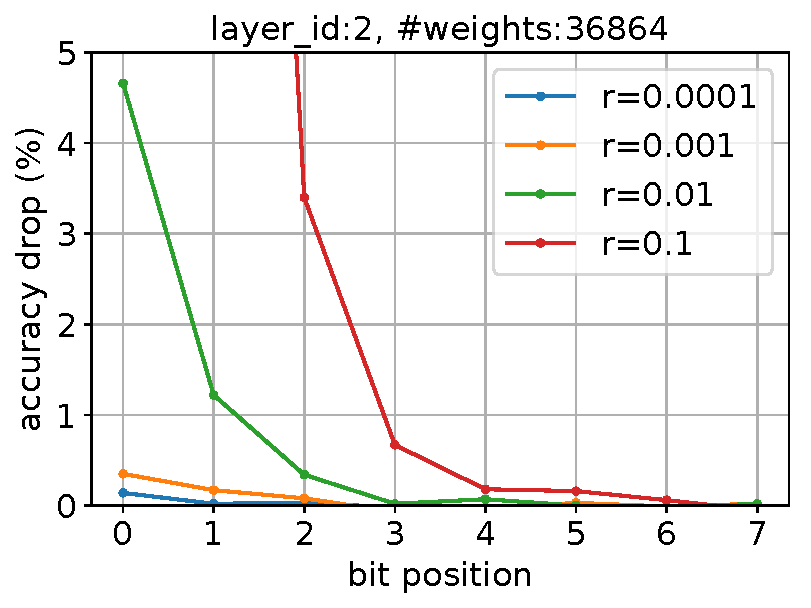
\includegraphics[width=\textwidth]{NeuRIPS2019/images/bit_significance/vgg16_2_int8_bit_significance.pdf}
		\caption{VGG16}
	\end{subfigure}
	\begin{subfigure}{.42\textwidth}
		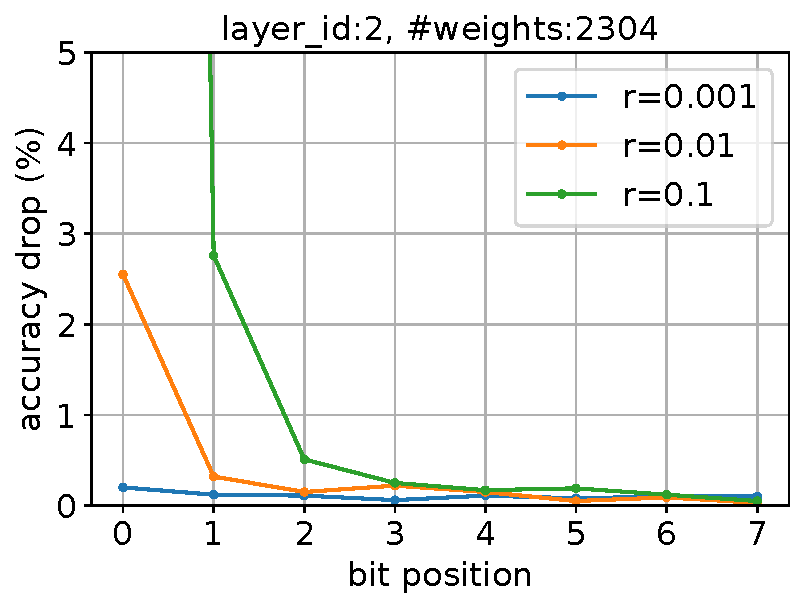
\includegraphics[width=\textwidth]{NeuRIPS2019/images/bit_significance/resnet56_2_int8_bit_significance.pdf}
		\caption{ResNet56}
	\end{subfigure}
	\caption{The accuracy drops of the DNNs with various fault rate at eight bit positions (0: MSB, 7: LSB). Faults are injected to only the second convolutional layer. Other layers show the similar pattern. Dataset is Cifar10.  }
	\label{fig:bit_significance}
\end{figure}

Figure~\ref{fig:bit_significance} shows the accuracy drops of the DNNs after injecting faults to different bit positions. The most significant bit cause the highest accuracy drops. This implies that bits of higher significance have the highest priority of error correction. On the contrary, the bits with a smaller weight causes negaliable or no accuracy drop to DNNs. 

The above observations lead to our in-place near-zero cost protection strategies that leverage existing ECC algorithms to provide protection guarantee while rely on the DNN-specific properties to lower storage overhead. The core idea is to use non-informative bits in DNN parameters to store check bits in-place. We next elaborate the protection mechanism. 

\subsection{Mechanism}
Our protection mechanism is based on several standalone protection methods. We first introduces these methods and then explain how to achieve adaptivity based on a given storage budget.  

\subsubsection{Lossy in-place protection}
Lossy inplace protection uses the least significant bit of each weight in a 64-bit long data block to store the check bits of SEC-DEC $[64, 57, 1]$ code. As the check bits are stored in-place, the to-be-protected weights and the generated code-word are of the same length. For example, when the number of check bits is seven, it is able to cover at most 57 number of bits ($k = 57$). These data bits can be the seven high bits for the first seven weights and all the eight bits for the last weight. 
This protection strategy brings no storage overhead but is likely to introduce accuracy drop because the encoding changes the last bit of some weights. 


\subsubsection{Lossless in-place protections}

Lossless in-place protections are two methods that use the non-informative bits in the significant bits of small values to store check bits. When a 8-bit quantized value is within the range of $[-64, 63]$, there is one significant bit available for check bits per weight. Thus, for a 64-bit long data block that contains eight weights, a SEC-DED $[64, 57, 1]$ code (\textit{ECC64} in short) can be used for single bit error correction in 64-bit long data. Similarly, if a value is within the range of $[-32, 31]$, codes with stronger protection capacity, such as a SEC-DED $[32, 26, 1]$ code (\textit{ECC32} in short) or a  BCH $[63, 51, 2]$ code (\textit{BCH} in short), can be applied for single bit error correction in 32-bit long data or double error correction in 64-bit long data respectively. As some of the weights have large values that are out of the above ranges, it is necessary to keep track of the indexes of large values so that the actual values can be recovered after decoding. 
Even though storing the indexes of large values bring some storage overhead, the overhead is negligible because the percentage of large values are small, as has illustrated in Table~\ref{tab:weight_distribution}.  

\subsubsection{Adaptive protection}
In-place adaptive near-zero cost protection chooses whether the lossy protection or one of the lossless protections is used to protect weights in a specific layer. Let $\overrightarrow{\mathbf{e}} = [e_1, \cdots, e_L], e_i \in \{0, 1, 2\}$, where $e_i = 0$ means the weights in the $i$-th layer are protected by the lossy approach while $e_i = 1, 2$ means they are protected by the lossless approaches. An adaptive protection aims to find the protection strategy $P$, represented as the row vector $\overrightarrow{\mathbf{e}}$, for the objective function in Eq.~\ref{eq:objective}. 

% Mathematically, let $\mathcal{A}(W)$ and $\mathcal{A}(W|\overrightarrow{\mathbf{e}})$ be the accuracy of the DNN on a task with parameters $W$ using fault-free memory and memory with protection scheme $\overrightarrow{\mathbf{e}}$ respectively. Let $N^b_i$ be the number of large values whose indexes need to be recorded in the lossless protection scheme. Let $L$ be the number of parameterized layers in a DNN. Adaptive protection is an optimization problem: 

% Previous objective: minimize overhead
% \begin{align}
%     & \min_{\overrightarrow{\mathbf{e}}} \sum_{i=1}^L e_i \times N^{b}_i,  \\
%     & s.t. \quad \mathcal{A}(W) - \mathcal{A}(W|\overrightarrow{\mathbf{e}}) < \alpha. 
% \end{align}
The problem is NP hard, provable through a reduction of the problem to the classic knapsack problem~\cite{hochba1997approximation}. We developed the following greedy algorithm to solve the problem efficiently. The steps are as follows:  
\begin{enumerate}
    \item Sort layers according to the overhead of storing the indexes of values out of range $[-64, 63]$ in an increasing order. Let $L$ be the number of layers. For each layer $l =1, \cdots, L$ in the sorted list, calculate the overhead of applying the lossless in-place \textit{ECC64} for layers up to $l$ (including $l$). If the overhead is over the budget $B$, then the protection strategy is to use the lossless in-place \textit{ECC64} for the layers up to $l-1$ and use the lossy in-place protection for the remaining layers. Otherwise, increase $l$. 
    \item Sort layers according to the overhead of storing the indexes of values out of range $[-32, 31]$ in an increasing order. For each layer $l =1, \cdots, L$ in the sorted list, calculate the overhead of applying the lossless in-place \textit{BCH} or $ECC32$ for layers up to $l$ (including $l$). If the overhead is over the budget $B$, then the protection strategy is to use the lossless in-place \textit{BCH} or \textit{ECC32} for the layers up to $l-1$ and use lossless in-place \textit{ECC64} for the remaining layers. Otherwise, increase $l$.
    
\end{enumerate}

The above steps require the calculation of the protection overhead. The exact overhead depends on the way to store the indexes of large values, which is elaborated next.   
\TODO{Do we need to include the header design? Should we put it here or in the hardware design section?}

\subsection{Hardware design}

Figure~\ref{fig:hardware} illustrate our proposed hardware design to support the protection mechanism. As show in Figure~\ref{fig:hardware}, we introduce two small changes to the existing ECC/BCH logic. The first change is a large value (LV) table, which encodes the locations of large weights within each tile as a bit vector. Each row in the LV table is an 8-bit vector corresponding to 8 weightsin a tile. For a 256-weight tile, this LV table has a size of 32 bytes.  The second change is the bit swizzling logic. According to our in-place ECC encoding scheme, the ECC bits are extracted and the 6th bit of each weight is recovered from the sign bit: replicated for small weights or inversed for large weights. (with regularized training, the large value table is no longer needed.) \TODO{Now we have ECC32, ECC64, BCH. Can we have the hardware to support all this? Too much area cost?}

\begin{figure}
    \centering
    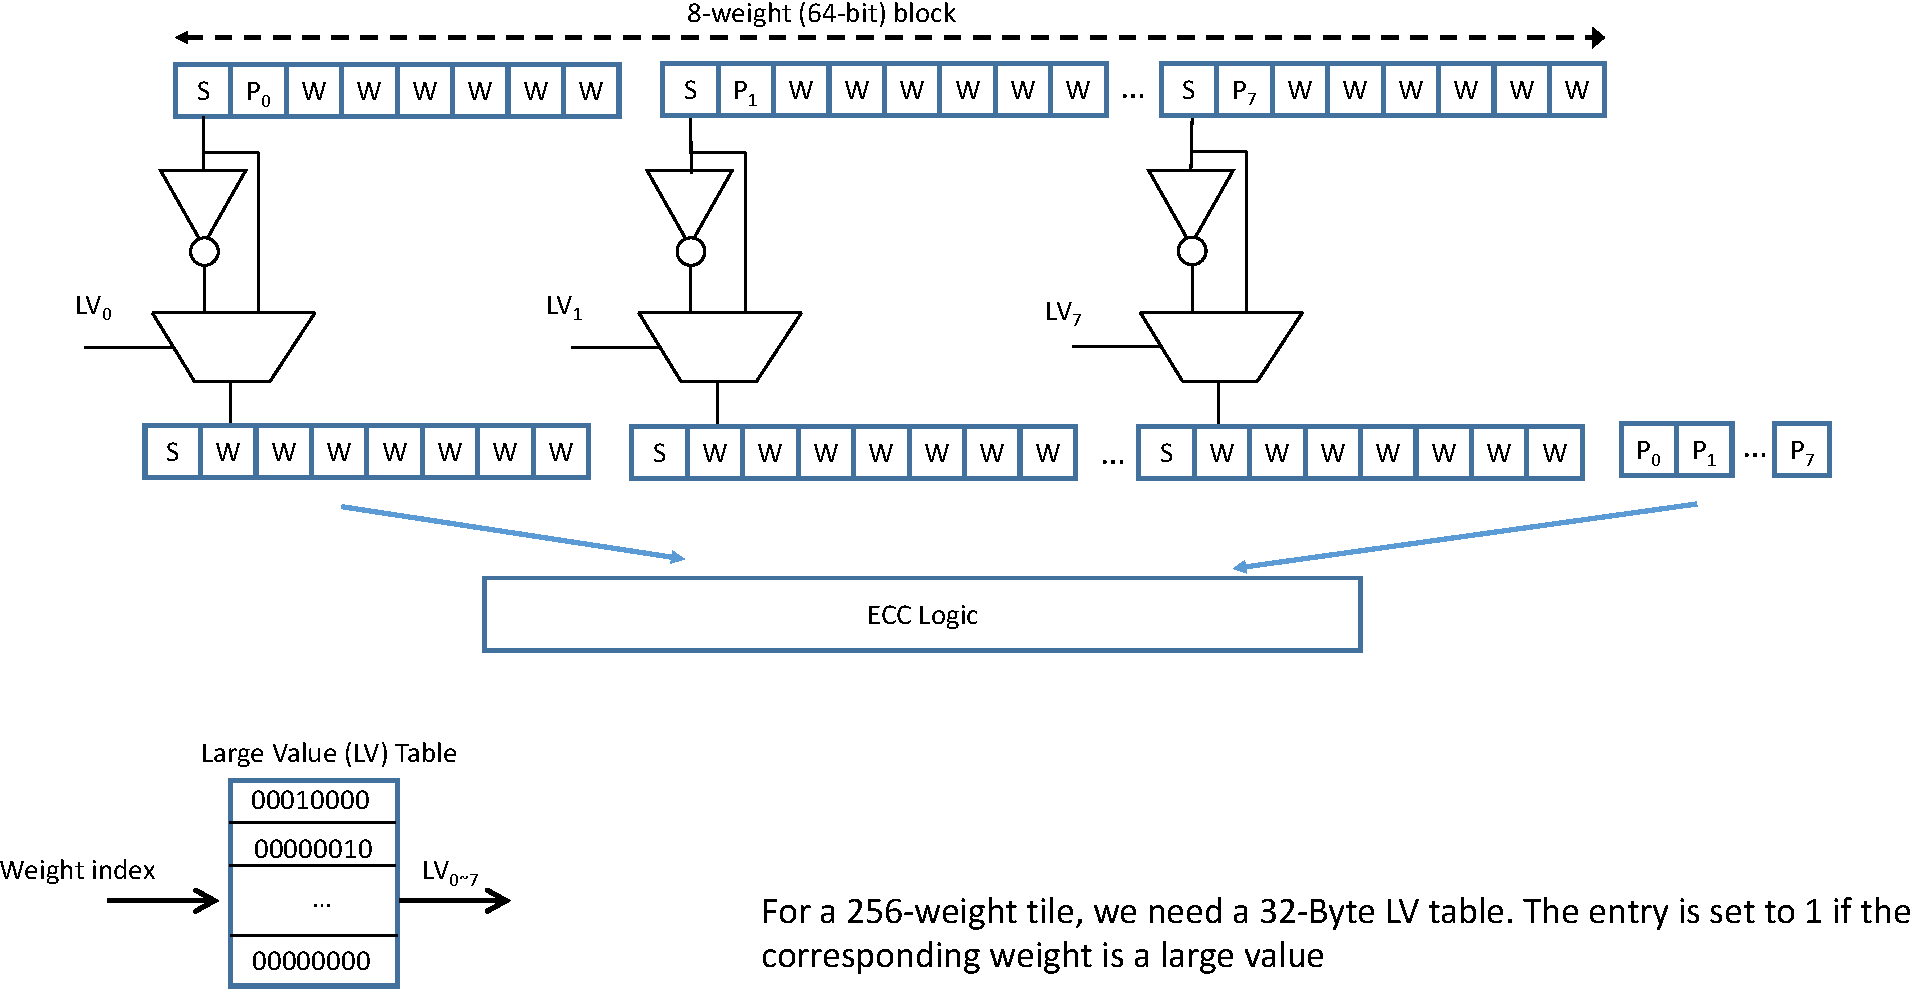
\includegraphics[width=0.99\textwidth]{NeuRIPS2019/images/hardware/DNN-ECC-crop.pdf}
    \caption{Hardware design for in-place ECC protection.\TODO{remove the text "for a 256-entry ...", it is for internal discussion. not a part of the design. Also, it would be helpful if the LV table can be move up so as to save some space}}
    \label{fig:hardware}
\end{figure}

  

\section{Evaluation}
We conducted a set of experiments to examine the efficacy of our proposed protection mechanisms by answering the following questions:
\begin{enumerate}
    \item How effective can the proposed strategies in protecting DNNs from memory faults?
    \item What is the overhead of the protection? 
\end{enumerate}

\subsection{Experiment settings}
\paragraph{Models and datasets}
We focus on convolutional neural networks in DNNs as they have shown great performance in many real-world applications. The models we used in the experiments include VGG16, ResNet18, and SqueezeNet. The three models cover a certain variety of popular CNNs. The accuracies of these models are listed in Table~\ref{tab:weight_distribution}. 

\paragraph{Counterparts for Comparisons}
\begin{itemize}
    \item \textbf{Parity Zero (zero):} It adds one parity bit to detect single bit error in a eight bit data block (e.g. a single weight parameter). Once errors are detected, the weight is set to zero. 
    \item \textbf{Parity Average (avg):} It sets the detected faulty weight to the average value of its left and right neighbors. 
    \item \textbf{Majority Vote (vote)} It uses 1-bit encoding to indicate whether a value is larger than 32 and protect the first three bits of a value less than 32 by majority vote. The storage overhead is the same as the Parity Zero/Average solution.  \TODO{This method is what we proposed. How to state it explicitly? Is it one of our contribution? }
    \item \textbf{SEC-DEC (ecc)} It is the traditional SEC-DEC $[72, 64, 1]$ code-based protection. 
    \item \textbf{Ours (adaptive)} This is our proposed in-place adaptive approach. Note that there are four corner cases of the protection: \textbf{Lossy}, \textbf{ECC64}, \textbf{ECC32}, and \textbf{BCH}  represent that every layer is encoded using the lossy in-place protection,  lossless in-place \textit{ECC64}, lossless in-place \textit{ECC32}, and lossless in-place \textit{BCH} respectively. 

\end{itemize}
% \paragraph{Machines}

\subsection{Results}

\begin{figure}
	\centering
	\begin{subfigure}{.3\textwidth}
		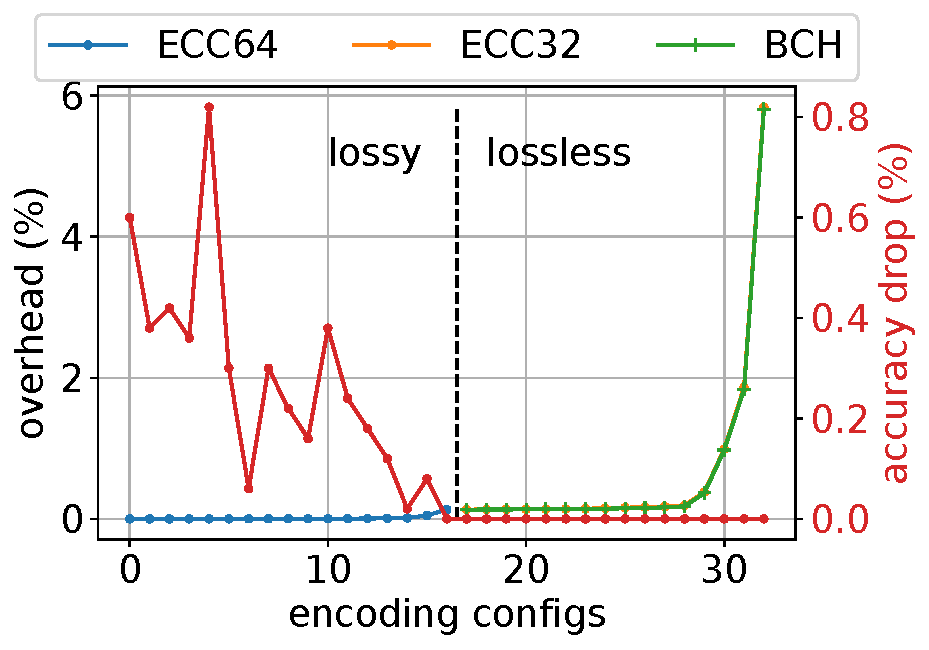
\includegraphics[width=\textwidth]{NeuRIPS2019/images/overhead/vgg16_int8_overhead.pdf}
		\caption{VGG16}
	\end{subfigure}
	\begin{subfigure}{.3\textwidth}
		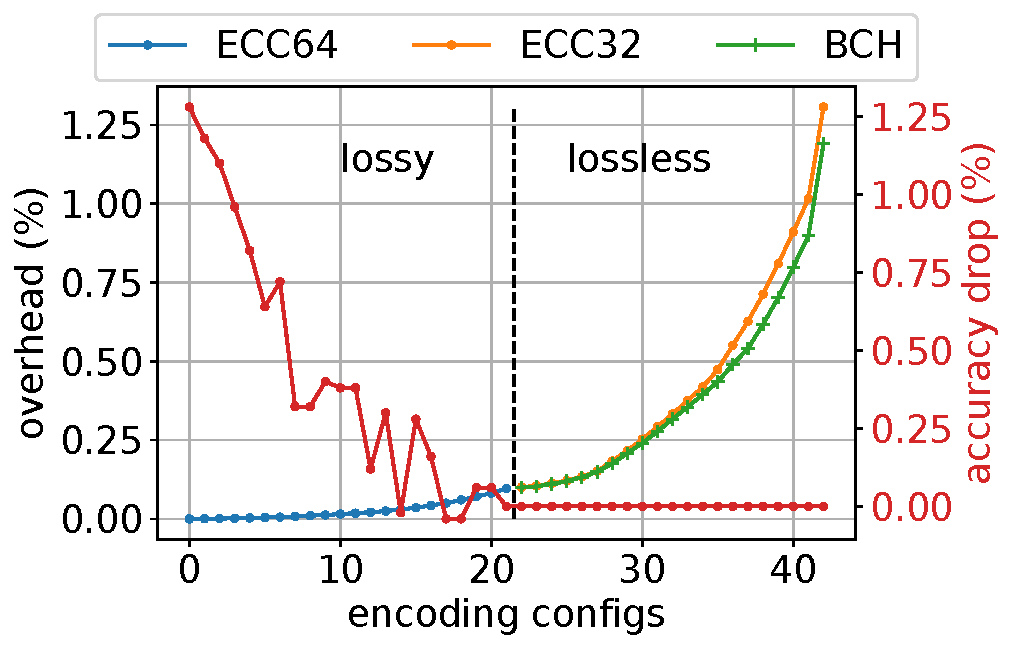
\includegraphics[width=\textwidth]{NeuRIPS2019/images/overhead/resnet18_int8_overhead.pdf}
		\caption{ResNet18}
	\end{subfigure}
	\begin{subfigure}{.3\textwidth}
		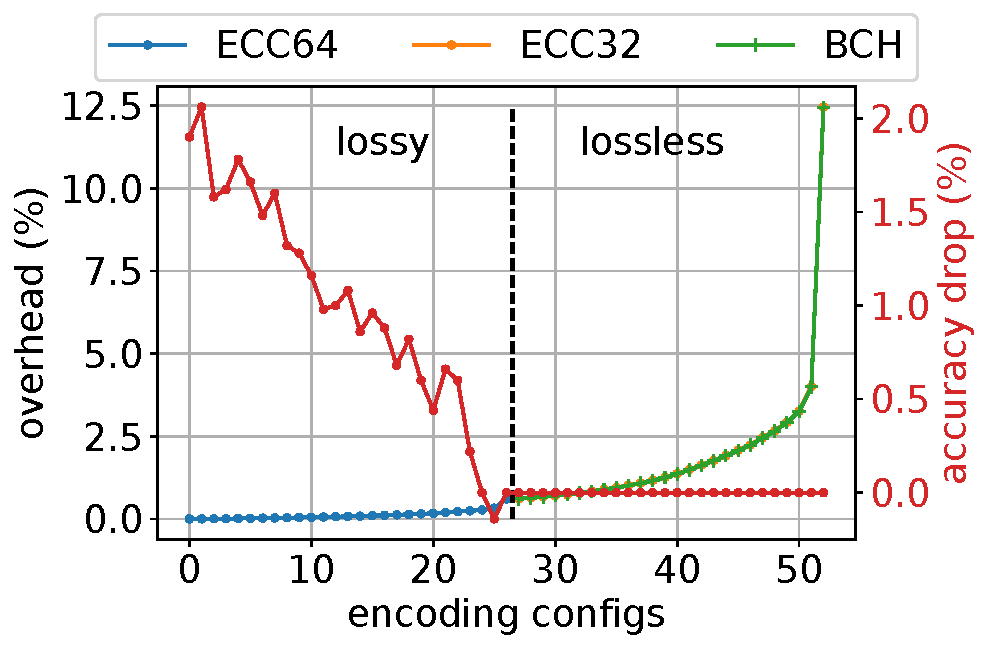
\includegraphics[width=\textwidth]{NeuRIPS2019/images/overhead/squeezenet_int8_overhead.pdf}
		\caption{SqueezeNet}
	\end{subfigure}
	\caption{Storage overhead.}
	\label{fig:overhead}
\end{figure}


\begin{figure}
	\centering
	\begin{subfigure}{.3\textwidth}
		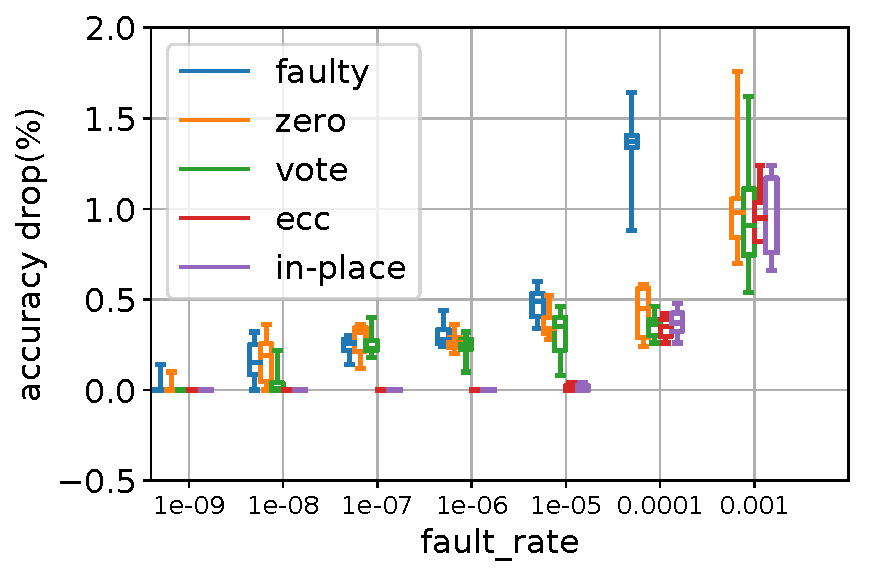
\includegraphics[width=\textwidth]{NeuRIPS2019/images/protection/vgg16_int8_accuracy_drop.pdf}
		\caption{VGG16}
	\end{subfigure}
	\begin{subfigure}{.3\textwidth}
		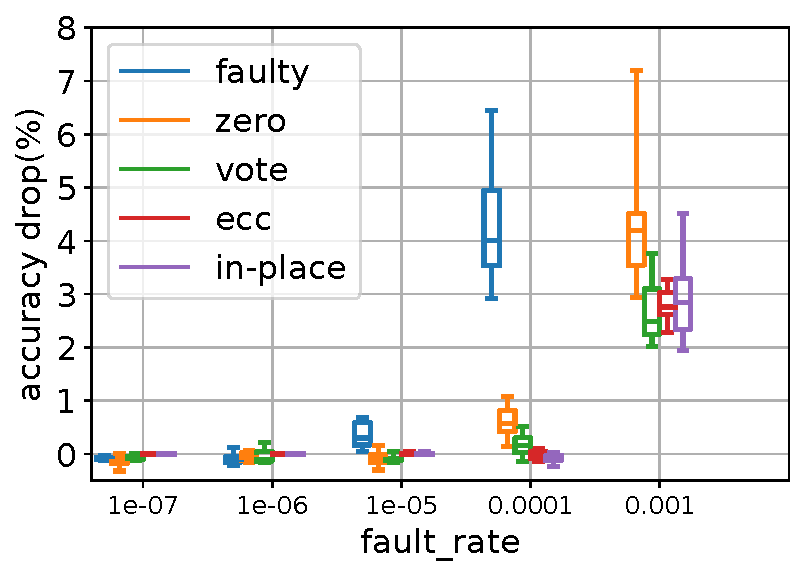
\includegraphics[width=\textwidth]{NeuRIPS2019/images/protection/resnet18_int8_accuracy_drop.pdf}
		\caption{ResNet18}
	\end{subfigure}
	\begin{subfigure}{.3\textwidth}
		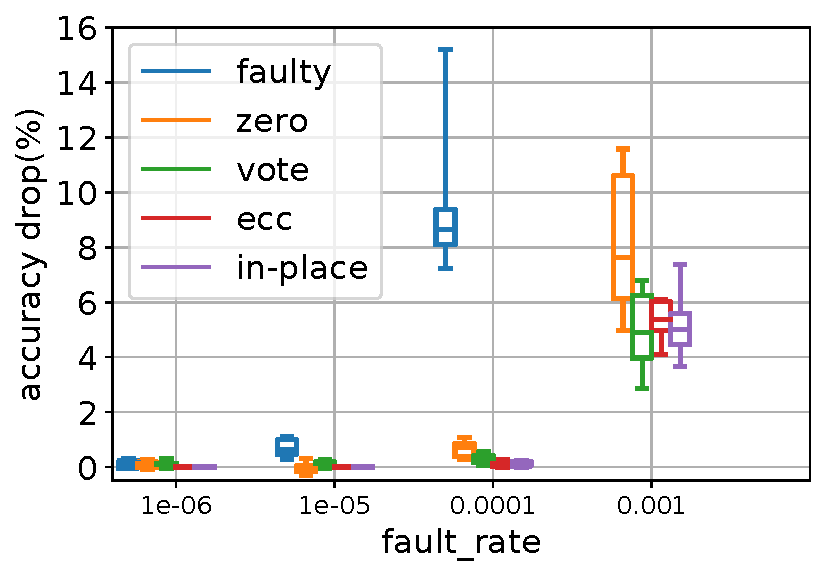
\includegraphics[width=\textwidth]{NeuRIPS2019/images/protection/squeezenet_int8_accuracy_drop.pdf}
		\caption{SqueezeNet}
	\end{subfigure}
	\caption{Accuracy drop with different protection strategies.}
	\label{fig:overhead}
\end{figure}


% Please add the following required packages to your document preamble:
% \usepackage{multirow}
\begin{table}[]
\centering 
\caption{Accuracy drop of VGG16 under different memory fault rate.}
\small 
\begin{tabular}{|l|l|l|l|l|l|l|}
\hline
\multirow{2}{*}{strategy} & \multirow{2}{*}{\begin{tabular}[c]{@{}l@{}}target \\ budget (\%)\end{tabular}} & \multirow{2}{*}{\begin{tabular}[c]{@{}l@{}}overhead\\ (\%)\end{tabular}} & \multicolumn{4}{l|}{accuracy drop (\%) under different fault rate} \\ \cline{4-7} 
 &  &  & 1e-06 & 1e-05 & 1e-04 & 1e-03 \\ \hline
faulty & - & 0 & 0.31 $\pm$ 0.1 & 0.48 $\pm$ 0.14 & 1.34 $\pm$ 0.37 & 22.5 $\pm$ 7.14 \\ \hline
zero & - & 12.5 & 0.27 $\pm$ 0.09 & 0.36 $\pm$ 0.1 & 0.52 $\pm$ 0.39 & 1.08 $\pm$ 0.38 \\ \hline
avg & - & 12.5 & 0.16 $\pm$ 0.13 & 0.27 $\pm$ 0.11 & 0.28 $\pm$ 0.12 & 0.33 $\pm$ 0.17 \\ \hline
vote & - & 12.5 & 0.24 $\pm$ 0.13 & 0.3 $\pm$ 0.14 & 0.34 $\pm$ 0.14 & 1.09 $\pm$ 0.62 \\ \hline
ecc & - & 12.5 & 0.0 $\pm$ 0.0 & 0.05 $\pm$ 0.09 & 0.36 $\pm$ 0.11 & 0.99 $\pm$ 0.34 \\ \hline
bch & - & 19.0 & 0.0 $\pm$ 0.0 & 0.0 $\pm$ 0.0 & 0.02 $\pm$ 0.08 & 0.3 $\pm$ 0.13 \\ \hline
\multirow{5}{*}{adaptive} & 0 (Lossy) & 0 & 0.6 $\pm$ 0.0 & 0.59 $\pm$ 0.04 & 0.54 $\pm$ 0.15 & 1.23 $\pm$ 0.41 \\ \cline{2-7} 
 & 0.13 (ECC64) & 0.13 & 0.0 $\pm$ 0.0 & 0.05 $\pm$ 0.09 & 0.37 $\pm$ 0.12 & 0.94 $\pm$ 0.3 \\ \cline{2-7} 
 & 1 & 0.98 & 0.0 $\pm$ 0.0 & 0.01 $\pm$ 0.01 & 0.06 $\pm$ 0.08 & 0.32 $\pm$ 0.14 \\ \cline{2-7} 
 & 2 & 1.84 & 0.0 $\pm$ 0.0 & 0.0 $\pm$ 0.0 & 0.03 $\pm$ 0.08 & 0.31 $\pm$ 0.19 \\ \cline{2-7} 
 & 5.81 (BCH) & 5.81 & 0.0 $\pm$ 0.0 & 0.0 $\pm$ 0.0 & 0.02 $\pm$ 0.05 & 0.32 $\pm$ 0.18 \\ \hline
\end{tabular}
\end{table}
\begin{table}[]
\centering 
\caption{Accuracy drop of ResNet16 under different memory fault rate.}
\small 
\begin{tabular}{|l|l|l|l|l|l|l|}
\hline
\multirow{2}{*}{strategy} & \multirow{2}{*}{\begin{tabular}[c]{@{}l@{}}target \\ budget (\%)\end{tabular}} & \multirow{2}{*}{\begin{tabular}[c]{@{}l@{}}overhead\\ (\%)\end{tabular}} & \multicolumn{4}{l|}{accuracy drop (\%) under different fault rate} \\ \cline{4-7} 
 &  &  & 1e-06 & 1e-05 & 1e-04 & 1e-03 \\ \hline
faulty & - & 0 & -0.07 $\pm$ 0.15 & 0.43 $\pm$ 0.48 & 4.56 $\pm$ 1.75 & 72.81 $\pm$ 2.1 \\ \hline
zero & - & 12.5 & -0.05 $\pm$ 0.09 & -0.08 $\pm$ 0.16 & 0.65 $\pm$ 0.49 & 4.73 $\pm$ 2.0 \\ \hline
avg & - & 12.5 & -0.08 $\pm$ 0.13 & 0.01 $\pm$ 0.12 & 0.63 $\pm$ 0.57 & 4.33 $\pm$ 1.2 \\ \hline
vote & - & 12.5 & -0.02 $\pm$ 0.23 & -0.09 $\pm$ 0.1 & 0.2 $\pm$ 0.31 & 3.14 $\pm$ 1.69 \\ \hline
ecc & - & 12.5 & 0.0 $\pm$ 0.0 & 0.0 $\pm$ 0.05 & -0.02 $\pm$ 0.1 & 2.81 $\pm$ 0.47 \\ \hline
bch & - & 19.0 & 0.0 $\pm$ 0.0 & 0.0 $\pm$ 0.0 & 0.0 $\pm$ 0.0 & 0.01 $\pm$ 0.13 \\ \hline
\multirow{5}{*}{adaptive} & 0 (Lossy) & 0 & 1.28 $\pm$ 0.0 & 1.26 $\pm$ 0.05 & 1.37 $\pm$ 0.19 & 4.0 $\pm$ 0.88 \\ \cline{2-7} 
 & 0.1 (ECC64) & 0.1 & 0.0 $\pm$ 0.0 & 0.0 $\pm$ 0.05 & -0.09 $\pm$ 0.12 & 3.04 $\pm$ 1.22 \\ \cline{2-7} 
 & 0.5 & 0.49 & 0.0 $\pm$ 0.0 & -0.01 $\pm$ 0.04 & -0.08 $\pm$ 0.09 & 0.54 $\pm$ 0.32 \\ \cline{2-7} 
 & 1.0 & 0.9 & 0.0 $\pm$ 0.0 & 0.0 $\pm$ 0.0 & 0.0 $\pm$ 0.06 & 0.07 $\pm$ 0.21 \\ \cline{2-7} 
 & 1.19 (BCH) & 1.19 & 0.0 $\pm$ 0.0 & 0.0 $\pm$ 0.0 & -0.02 $\pm$ 0.05 & 0.04 $\pm$ 0.15 \\ \hline
\end{tabular}
\end{table}
\begin{table}[]
\centering 
\caption{Accuracy drop of SqueezeNet under different memory fault rate.}
\small 
\begin{tabular}{|l|l|l|l|l|l|l|}
\hline
\multirow{2}{*}{strategy} & \multirow{2}{*}{\begin{tabular}[c]{@{}l@{}}target \\ budget (\%)\end{tabular}} & \multirow{2}{*}{\begin{tabular}[c]{@{}l@{}}overhead\\ (\%)\end{tabular}} & \multicolumn{4}{l|}{accuracy drop (\%) under different fault rate} \\ \cline{4-7} 
 &  &  & 1e-06 & 1e-05 & 1e-04 & 1e-03 \\ \hline
faulty & - & 0 & 0.1 $\pm$ 0.21 & 1.12 $\pm$ 1.67 & 10.07 $\pm$ 3.64 & 64.55 $\pm$ 1.62 \\ \hline
zero & - & 12.5 & 0.1 $\pm$ 0.19 & 0.09 $\pm$ 0.59 & 0.66 $\pm$ 0.34 & 8.21 $\pm$ 2.67 \\ \hline
avg & - & 12.5 & 0.13 $\pm$ 0.19 & 0.41 $\pm$ 0.76 & 0.87 $\pm$ 0.5 & 11.88 $\pm$ 4.75 \\ \hline
vote & - & 12.5 & 0.12 $\pm$ 0.14 & 0.11 $\pm$ 0.13 & 0.31 $\pm$ 0.25 & 5.27 $\pm$ 2.24 \\ \hline
ecc & - & 12.5 & 0.0 $\pm$ 0.0 & 0.0 $\pm$ 0.0 & 0.12 $\pm$ 0.12 & 6.98 $\pm$ 5.4 \\ \hline
bch & - & 19.0 & 0.0 $\pm$ 0.0 & 0.0 $\pm$ 0.0 & 0.0 $\pm$ 0.0 & 0.55 $\pm$ 0.76 \\ \hline
\multirow{5}{*}{adaptive} & 0 (Lossy) & 0 & 1.9 $\pm$ 0.0 & 1.9 $\pm$ 0.0 & 2.05 $\pm$ 0.18 & 9.48 $\pm$ 6.67 \\ \cline{2-7} 
 & 0.6 (ECC64) & 0.6 & 0.0 $\pm$ 0.0 & 0.0 $\pm$ 0.0 & 0.12 $\pm$ 0.12 & 5.31 $\pm$ 1.84 \\ \cline{2-7} 
 & 2 & 0.91 & 0.0 $\pm$ 0.0 & 0.0 $\pm$ 0.0 & 0.17 $\pm$ 0.19 & 1.43 $\pm$ 0.62 \\ \cline{2-7} 
 & 4 & 3.99 & 0.0 $\pm$ 0.0 & 0.0 $\pm$ 0.0 & 0.0 $\pm$ 0.0 & 0.35 $\pm$ 0.23 \\ \cline{2-7} 
 & 12.45 (BCH) & 12.45 & 0.0 $\pm$ 0.0 & 0.0 $\pm$ 0.0 & 0.0 $\pm$ 0.0 & 0.2 $\pm$ 0.29 \\ \hline
\end{tabular}
\end{table}

\subsection{Discussion}
\TODO{Aonther quick look at the big picture: what we are proposing so far is to replace standard ECC with special in-place ECC and large weight indices. The advantage is the reduced storage overhead, which is at most 12.5\%. This is significant for large networks. But the percentage is somewhat limited and we still need the ECC hardware with minor additional logic.

Other schemes like majority voting and delta (and other in-place coding) are more suitable for software, which would eliminate the need for ECC hardware along with the ECC storage overhead. But they are not as good as ECC when the error rate is high.}
\section{Conclusion}

\bibliography{bib} 
\bibliographystyle{plain}


\appendix

\section{ADMM Regularization}

\TODO{probably want to consider training with large value position regularization.}

Let $W_i$ and $W_i^q$ be the weights before and after 8-bit quantization in the $i$-th convolutional layer. 
The loss function subject to some constraints on the weights:
\begin{align}
    & \min_{W_i^q, b_i} f(\{W_i^q\}_{i=1}^{L}, \{b_i^q\}_{i=1}^L) \\
    & s.t. \quad W_i^q \in S_i, i = 1, \cdots, L 
\end{align}

The weights are a four-dimensional tensor. If flattened, it is a vector of length $A_i\times C_i \times H_i \times W_i$, where $A_i$, $C_i$, $H_i$ and $W_i$ are respectively the number of filters, the number of channels in a filter, the height of the filter, and the width of the filter, in the $i$-th convolutional layer. 

To regulate the position of large values in weights, the constraint on the weights in the $i$-th convolutional layer is given by $S_i = \{X|$ the first $k$ number of elements in every $n$-element block can only have a value in the range of $[-Q_{max}/2^m, Q_{max}/2^m)\}$, where $Q_{max}$ is the maximum quantized value. For example, in case $n=8$, $k=7$, $m=1$ and $Q_{max}=128$, the eight-element block can use inplace SEC-DED of code $[64, 57]$ by storing the $7$ check bits in the first 7 elements. 

To formalize the problem in ADMM, let 
$g_i(W_i^q) = \begin{cases}
    0,& \text{if } W_i^q \in S_i\\
    +\infty,              & \text{otherwise}.
\end{cases}$. The optimization problem becomes:
\begin{align}
    & \min_{W_i^q, b_i} f(\{W_i^q\}_{i=1}^{L}, \{b_i^q\}_{i=1}^L) + \sum_{i=1}^{L}{g_i(Z_i)}, \\
    & s.t. \quad W_i^q = Z_i, i = 1, \cdots, L 
\end{align}

ADMM alternates between the optimization of $W_i^q$, $b_i^q$ (also the floating-point version $W_i$ and $b_i$) and $Z_i$.


% \section{General formatting instructions}
% \label{gen_inst}

% The text must be confined within a rectangle 5.5~inches (33~picas) wide and
% 9~inches (54~picas) long. The left margin is 1.5~inch (9~picas).  Use 10~point
% type with a vertical spacing (leading) of 11~points.  Times New Roman is the
% preferred typeface throughout, and will be selected for you by default.
% Paragraphs are separated by \nicefrac{1}{2}~line space (5.5 points), with no
% indentation.

% The paper title should be 17~point, initial caps/lower case, bold, centered
% between two horizontal rules. The top rule should be 4~points thick and the
% bottom rule should be 1~point thick. Allow \nicefrac{1}{4}~inch space above and
% below the title to rules. All pages should start at 1~inch (6~picas) from the
% top of the page.

% For the final version, authors' names are set in boldface, and each name is
% centered above the corresponding address. The lead author's name is to be listed
% first (left-most), and the co-authors' names (if different address) are set to
% follow. If there is only one co-author, list both author and co-author side by
% side.

% Please pay special attention to the instructions in Section \ref{others}
% regarding figures, tables, acknowledgments, and references.

% \section{Headings: first level}
% \label{headings}

% All headings should be lower case (except for first word and proper nouns),
% flush left, and bold.

% First-level headings should be in 12-point type.

% \subsection{Headings: second level}

% Second-level headings should be in 10-point type.

% \subsubsection{Headings: third level}

% Third-level headings should be in 10-point type.

% \paragraph{Paragraphs}

% There is also a \verb+\paragraph+ command available, which sets the heading in
% bold, flush left, and inline with the text, with the heading followed by 1\,em
% of space.

% \section{Citations, figures, tables, references}
% \label{others}

% These instructions apply to everyone.

% \subsection{Citations within the text}

% The \verb+natbib+ package will be loaded for you by default.  Citations may be
% author/year or numeric, as long as you maintain internal consistency.  As to the
% format of the references themselves, any style is acceptable as long as it is
% used consistently.

% The documentation for \verb+natbib+ may be found at
% \begin{center}
%   \url{http://mirrors.ctan.org/macros/latex/contrib/natbib/natnotes.pdf}
% \end{center}
% Of note is the command \verb+\citet+, which produces citations appropriate for
% use in inline text.  For example,
% \begin{verbatim}
%   \citet{hasselmo} investigated\dots
% \end{verbatim}
% produces
% \begin{quote}
%   Hasselmo, et al.\ (1995) investigated\dots
% \end{quote}

% If you wish to load the \verb+natbib+ package with options, you may add the
% following before loading the \verb+neurips_2019+ package:
% \begin{verbatim}
%   \PassOptionsToPackage{options}{natbib}
% \end{verbatim}

% If \verb+natbib+ clashes with another package you load, you can add the optional
% argument \verb+nonatbib+ when loading the style file:
% \begin{verbatim}
%   \usepackage[nonatbib]{neurips_2019}
% \end{verbatim}

% As submission is double blind, refer to your own published work in the third
% person. That is, use ``In the previous work of Jones et al.\ [4],'' not ``In our
% previous work [4].'' If you cite your other papers that are not widely available
% (e.g., a journal paper under review), use anonymous author names in the
% citation, e.g., an author of the form ``A.\ Anonymous.''

% \subsection{Footnotes}

% Footnotes should be used sparingly.  If you do require a footnote, indicate
% footnotes with a number\footnote{Sample of the first footnote.} in the
% text. Place the footnotes at the bottom of the page on which they appear.
% Precede the footnote with a horizontal rule of 2~inches (12~picas).

% Note that footnotes are properly typeset \emph{after} punctuation
% marks.\footnote{As in this example.}

% \subsection{Figures}

% \begin{figure}
%   \centering
%   \fbox{\rule[-.5cm]{0cm}{4cm} \rule[-.5cm]{4cm}{0cm}}
%   \caption{Sample figure caption.}
% \end{figure}

% All artwork must be neat, clean, and legible. Lines should be dark enough for
% purposes of reproduction. The figure number and caption always appear after the
% figure. Place one line space before the figure caption and one line space after
% the figure. The figure caption should be lower case (except for first word and
% proper nouns); figures are numbered consecutively.

% You may use color figures.  However, it is best for the figure captions and the
% paper body to be legible if the paper is printed in either black/white or in
% color.

% \subsection{Tables}

% All tables must be centered, neat, clean and legible.  The table number and
% title always appear before the table.  See Table~\ref{sample-table}.

% Place one line space before the table title, one line space after the
% table title, and one line space after the table. The table title must
% be lower case (except for first word and proper nouns); tables are
% numbered consecutively.

% Note that publication-quality tables \emph{do not contain vertical rules.} We
% strongly suggest the use of the \verb+booktabs+ package, which allows for
% typesetting high-quality, professional tables:
% \begin{center}
%   \url{https://www.ctan.org/pkg/booktabs}
% \end{center}
% This package was used to typeset Table~\ref{sample-table}.

% \begin{table}
%   \caption{Sample table title}
%   \label{sample-table}
%   \centering
%   \begin{tabular}{lll}
%     \toprule
%     \multicolumn{2}{c}{Part}                   \\
%     \cmidrule(r){1-2}
%     Name     & Description     & Size ($\mu$m) \\
%     \midrule
%     Dendrite & Input terminal  & $\sim$100     \\
%     Axon     & Output terminal & $\sim$10      \\
%     Soma     & Cell body       & up to $10^6$  \\
%     \bottomrule
%   \end{tabular}
% \end{table}

% \section{Final instructions}

% Do not change any aspects of the formatting parameters in the style files.  In
% particular, do not modify the width or length of the rectangle the text should
% fit into, and do not change font sizes (except perhaps in the
% \textbf{References} section; see below). Please note that pages should be
% numbered.

% \section{Preparing PDF files}

% Please prepare submission files with paper size ``US Letter,'' and not, for
% example, ``A4.''

% Fonts were the main cause of problems in the past years. Your PDF file must only
% contain Type 1 or Embedded TrueType fonts. Here are a few instructions to
% achieve this.

% \begin{itemize}

% \item You should directly generate PDF files using \verb+pdflatex+.

% \item You can check which fonts a PDF files uses.  In Acrobat Reader, select the
%   menu Files$>$Document Properties$>$Fonts and select Show All Fonts. You can
%   also use the program \verb+pdffonts+ which comes with \verb+xpdf+ and is
%   available out-of-the-box on most Linux machines.

% \item The IEEE has recommendations for generating PDF files whose fonts are also
%   acceptable for NeurIPS. Please see
%   \url{http://www.emfield.org/icuwb2010/downloads/IEEE-PDF-SpecV32.pdf}

% \item \verb+xfig+ "patterned" shapes are implemented with bitmap fonts.  Use
%   "solid" shapes instead.

% \item The \verb+\bbold+ package almost always uses bitmap fonts.  You should use
%   the equivalent AMS Fonts:
% \begin{verbatim}
%   \usepackage{amsfonts}
% \end{verbatim}
% followed by, e.g., \verb+\mathbb{R}+, \verb+\mathbb{N}+, or \verb+\mathbb{C}+
% for $\mathbb{R}$, $\mathbb{N}$ or $\mathbb{C}$.  You can also use the following
% workaround for reals, natural and complex:
% \begin{verbatim}
%   \newcommand{\RR}{I\!\!R} %real numbers
%   \newcommand{\Nat}{I\!\!N} %natural numbers
%   \newcommand{\CC}{I\!\!\!\!C} %complex numbers
% \end{verbatim}
% Note that \verb+amsfonts+ is automatically loaded by the \verb+amssymb+ package.

% \end{itemize}

% If your file contains type 3 fonts or non embedded TrueType fonts, we will ask
% you to fix it.

% \subsection{Margins in \LaTeX{}}

% Most of the margin problems come from figures positioned by hand using
% \verb+\special+ or other commands. We suggest using the command
% \verb+\includegraphics+ from the \verb+graphicx+ package. Always specify the
% figure width as a multiple of the line width as in the example below:
% \begin{verbatim}
%   \usepackage[pdftex]{graphicx} ...
%   \includegraphics[width=0.8\linewidth]{myfile.pdf}
% \end{verbatim}
% See Section 4.4 in the graphics bundle documentation
% (\url{http://mirrors.ctan.org/macros/latex/required/graphics/grfguide.pdf})

% A number of width problems arise when \LaTeX{} cannot properly hyphenate a
% line. Please give LaTeX hyphenation hints using the \verb+\-+ command when
% necessary.

% \subsubsection*{Acknowledgments}

% Use unnumbered third level headings for the acknowledgments. All acknowledgments
% go at the end of the paper. Do not include acknowledgments in the anonymized
% submission, only in the final paper.

% \section*{References}

% References follow the acknowledgments. Use unnumbered first-level heading for
% the references. Any choice of citation style is acceptable as long as you are
% consistent. It is permissible to reduce the font size to \verb+small+ (9 point)
% when listing the references. {\bf Remember that you can use more than eight
%   pages as long as the additional pages contain \emph{only} cited references.}
% \medskip

% \small

% [1] Alexander, J.A.\ \& Mozer, M.C.\ (1995) Template-based algorithms for
% connectionist rule extraction. In G.\ Tesauro, D.S.\ Touretzky and T.K.\ Leen
% (eds.), {\it Advances in Neural Information Processing Systems 7},
% pp.\ 609--616. Cambridge, MA: MIT Press.

% [2] Bower, J.M.\ \& Beeman, D.\ (1995) {\it The Book of GENESIS: Exploring
%   Realistic Neural Models with the GEneral NEural SImulation System.}  New York:
% TELOS/Springer--Verlag.

% [3] Hasselmo, M.E., Schnell, E.\ \& Barkai, E.\ (1995) Dynamics of learning and
% recall at excitatory recurrent synapses and cholinergic modulation in rat
% hippocampal region CA3. {\it Journal of Neuroscience} {\bf 15}(7):5249-5262.

\end{document}
